


\tikzset{every picture/.style={line width=0.75pt}} %set default line width to 0.75pt        

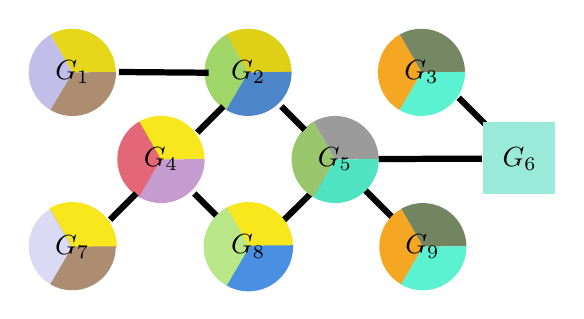
\begin{tikzpicture}[x=0.75pt,y=0.75pt,yscale=-0.7,xscale=0.7]
%uncomment if require: \path (0,1438); %set diagram left start at 0, and has height of 1438

%Straight Lines [id:da4750966694185179] 
\draw [color={rgb, 255:red, 0; green, 0; blue, 0 }  ,draw opacity=1 ][line width=2.25]    (252,1020) -- (272,1040) ;
%Straight Lines [id:da5150276886008835] 
\draw [color={rgb, 255:red, 0; green, 0; blue, 0 }  ,draw opacity=1 ][line width=2.25]    (312,1040) -- (342,1010.31) ;
%Straight Lines [id:da4895817670375473] 
\draw [color={rgb, 255:red, 0; green, 0; blue, 0 }  ,draw opacity=1 ][line width=2.25]    (362,1010) -- (392,1040) ;
%Straight Lines [id:da8896491664010189] 
\draw [color={rgb, 255:red, 0; green, 0; blue, 0 }  ,draw opacity=1 ][line width=2.25]    (378.8,996.26) -- (450,996) ;
%Shape: Pie [id:dp15959605123169607] 
\draw  [draw opacity=0][fill={rgb, 255:red, 248; green, 231; blue, 28 }  ,fill opacity=1 ] (214.1,970.48) .. controls (218.49,967.96) and (223.58,966.52) .. (229,966.52) .. controls (245.48,966.52) and (258.86,979.81) .. (259,996.26) -- (229,996.52) -- cycle ;
%Shape: Pie [id:dp7541674422286544] 
\draw  [draw opacity=0][fill={rgb, 255:red, 170; green, 106; blue, 183 }  ,fill opacity=0.67 ] (259.19,996.28) .. controls (259.19,996.37) and (259.19,996.47) .. (259.19,996.57) .. controls (259.19,1013.14) and (245.76,1026.57) .. (229.19,1026.57) .. controls (223.62,1026.57) and (218.39,1025.05) .. (213.92,1022.4) -- (229.19,996.57) -- cycle ;
%Shape: Pie [id:dp5711882691598997] 
\draw  [draw opacity=0][fill={rgb, 255:red, 208; green, 2; blue, 27 }  ,fill opacity=0.6 ] (213.92,1022.4) .. controls (205.03,1017.19) and (199.06,1007.54) .. (199.06,996.49) .. controls (199.06,985.37) and (205.11,975.66) .. (214.1,970.48) -- (229.06,996.49) -- cycle ;
%Shape: Pie [id:dp06487384610910718] 
\draw  [draw opacity=0][fill={rgb, 255:red, 155; green, 155; blue, 155 }  ,fill opacity=1 ] (334.04,970.56) .. controls (338.43,968.04) and (343.52,966.6) .. (348.94,966.6) .. controls (365.42,966.6) and (378.8,979.89) .. (378.94,996.34) -- (348.94,996.6) -- cycle ;
%Shape: Pie [id:dp7524611065236799] 
\draw  [draw opacity=0][fill={rgb, 255:red, 80; green, 227; blue, 194 }  ,fill opacity=1 ] (379,996.28) .. controls (379,996.37) and (379,996.47) .. (379,996.57) .. controls (379,1013.14) and (365.57,1026.57) .. (349,1026.57) .. controls (343.42,1026.57) and (338.2,1025.05) .. (333.73,1022.4) -- (349,996.57) -- cycle ;
%Shape: Pie [id:dp59207049369319] 
\draw  [draw opacity=0][fill={rgb, 255:red, 153; green, 197; blue, 108 }  ,fill opacity=1 ] (333.86,1022.48) .. controls (324.97,1017.27) and (319,1007.62) .. (319,996.57) .. controls (319,985.45) and (325.05,975.74) .. (334.04,970.56) -- (349,996.57) -- cycle ;
%Shape: Pie [id:dp22947674130855522] 
\draw  [draw opacity=0][fill={rgb, 255:red, 34; green, 61; blue, 3 }  ,fill opacity=0.63 ] (394.43,1030.54) .. controls (398.82,1028.02) and (403.91,1026.58) .. (409.33,1026.58) .. controls (425.81,1026.58) and (439.18,1039.87) .. (439.33,1056.31) -- (409.33,1056.58) -- cycle ;
%Shape: Pie [id:dp2835887548099052] 
\draw  [draw opacity=0][fill={rgb, 255:red, 90; green, 242; blue, 208 }  ,fill opacity=1 ] (439.33,1056.31) .. controls (439.33,1056.41) and (439.33,1056.51) .. (439.33,1056.6) .. controls (439.33,1073.17) and (425.9,1086.6) .. (409.33,1086.6) .. controls (403.75,1086.6) and (398.53,1085.08) .. (394.06,1082.43) -- (409.33,1056.6) -- cycle ;
%Shape: Pie [id:dp13060561720498276] 
\draw  [draw opacity=0][fill={rgb, 255:red, 245; green, 166; blue, 35 }  ,fill opacity=1 ] (394.25,1082.45) .. controls (385.36,1077.24) and (379.39,1067.59) .. (379.39,1056.54) .. controls (379.39,1045.42) and (385.44,1035.72) .. (394.43,1030.54) -- (409.39,1056.54) -- cycle ;
%Shape: Pie [id:dp25936104896268675] 
\draw  [color={rgb, 255:red, 248; green, 231; blue, 28 }  ,draw opacity=1 ][fill={rgb, 255:red, 248; green, 231; blue, 28 }  ,fill opacity=1 ] (274.43,1030.54) .. controls (278.82,1028.02) and (283.91,1026.58) .. (289.33,1026.58) .. controls (305.81,1026.58) and (319.18,1039.87) .. (319.33,1056.31) -- (289.33,1056.58) -- cycle ;
%Shape: Pie [id:dp18697217704809055] 
\draw  [color={rgb, 255:red, 74; green, 144; blue, 226 }  ,draw opacity=1 ][fill={rgb, 255:red, 74; green, 144; blue, 226 }  ,fill opacity=1 ] (319.33,1056.31) .. controls (319.33,1056.41) and (319.33,1056.51) .. (319.33,1056.6) .. controls (319.33,1073.17) and (305.9,1086.6) .. (289.33,1086.6) .. controls (283.75,1086.6) and (278.53,1085.08) .. (274.06,1082.43) -- (289.33,1056.6) -- cycle ;
%Shape: Pie [id:dp8724690316630832] 
\draw  [color={rgb, 255:red, 185; green, 231; blue, 136 }  ,draw opacity=1 ][fill={rgb, 255:red, 185; green, 231; blue, 136 }  ,fill opacity=1 ] (274.06,1082.43) .. controls (265.17,1077.22) and (259.19,1067.57) .. (259.19,1056.52) .. controls (259.19,1045.4) and (265.24,1035.7) .. (274.23,1030.52) -- (289.19,1056.52) -- cycle ;
%Shape: Pie [id:dp4015988811299751] 
\draw  [draw opacity=0][fill={rgb, 255:red, 34; green, 61; blue, 3 }  ,fill opacity=0.62 ] (393.43,910.56) .. controls (397.82,908.04) and (402.91,906.6) .. (408.33,906.6) .. controls (424.81,906.6) and (438.19,919.89) .. (438.33,936.34) -- (408.33,936.6) -- cycle ;
%Shape: Pie [id:dp6392181041712679] 
\draw  [draw opacity=0][fill={rgb, 255:red, 90; green, 242; blue, 208 }  ,fill opacity=1 ] (438.33,936.31) .. controls (438.33,936.41) and (438.33,936.51) .. (438.33,936.6) .. controls (438.33,953.17) and (424.9,966.6) .. (408.33,966.6) .. controls (402.75,966.6) and (397.53,965.08) .. (393.06,962.43) -- (408.33,936.6) -- cycle ;
%Shape: Pie [id:dp04268417484462428] 
\draw  [draw opacity=0][fill={rgb, 255:red, 245; green, 166; blue, 35 }  ,fill opacity=1 ] (393.25,962.48) .. controls (384.36,957.27) and (378.39,947.62) .. (378.39,936.57) .. controls (378.39,925.45) and (384.44,915.74) .. (393.43,910.56) -- (408.39,936.57) -- cycle ;
%Shape: Pie [id:dp2303075286248355] 
\draw  [draw opacity=0][fill={rgb, 255:red, 222; green, 207; blue, 23 }  ,fill opacity=1 ] (274.1,910.54) .. controls (278.49,908.02) and (283.58,906.58) .. (289,906.58) .. controls (305.48,906.58) and (318.86,919.87) .. (319,936.31) -- (289,936.58) -- cycle ;
%Shape: Pie [id:dp8616807370257602] 
\draw  [draw opacity=0][fill={rgb, 255:red, 76; green, 133; blue, 200 }  ,fill opacity=1 ] (319,936.31) .. controls (319,936.41) and (319,936.51) .. (319,936.6) .. controls (319,953.17) and (305.57,966.6) .. (289,966.6) .. controls (283.42,966.6) and (278.2,965.08) .. (273.73,962.43) -- (289,936.6) -- cycle ;
%Shape: Pie [id:dp043769946944892446] 
\draw  [draw opacity=0][fill={rgb, 255:red, 159; green, 214; blue, 103 }  ,fill opacity=1 ] (273.92,962.45) .. controls (265.03,957.24) and (259.06,947.59) .. (259.06,936.54) .. controls (259.06,925.42) and (265.11,915.72) .. (274.1,910.54) -- (289.06,936.54) -- cycle ;
%Shape: Pie [id:dp5705398645606532] 
\draw  [draw opacity=0][fill={rgb, 255:red, 231; green, 215; blue, 27 }  ,fill opacity=1 ] (153.1,910.56) .. controls (157.49,908.04) and (162.58,906.6) .. (168,906.6) .. controls (184.48,906.6) and (197.86,919.89) .. (198,936.34) -- (168,936.6) -- cycle ;
%Shape: Pie [id:dp7072389331728437] 
\draw  [draw opacity=0][fill={rgb, 255:red, 173; green, 141; blue, 113 }  ,fill opacity=1 ] (198.19,936.36) .. controls (198.19,936.45) and (198.19,936.55) .. (198.19,936.65) .. controls (198.19,953.22) and (184.76,966.65) .. (168.19,966.65) .. controls (162.62,966.65) and (157.39,965.13) .. (152.92,962.48) -- (168.19,936.65) -- cycle ;
%Shape: Pie [id:dp8158973417554063] 
\draw  [draw opacity=0][fill={rgb, 255:red, 193; green, 191; blue, 234 }  ,fill opacity=1 ][line width=0.75]  (152.92,962.48) .. controls (144.03,957.27) and (138.06,947.62) .. (138.06,936.57) .. controls (138.06,925.45) and (144.11,915.74) .. (153.1,910.56) -- (168.06,936.57) -- cycle ;
%Shape: Pie [id:dp3241766948162095] 
\draw  [color={rgb, 255:red, 248; green, 231; blue, 28 }  ,draw opacity=1 ][fill={rgb, 255:red, 248; green, 231; blue, 28 }  ,fill opacity=1 ] (153.1,1030.56) .. controls (157.49,1028.04) and (162.58,1026.6) .. (168,1026.6) .. controls (184.48,1026.6) and (197.86,1039.89) .. (198,1056.34) -- (168,1056.6) -- cycle ;
%Shape: Pie [id:dp47660672298161044] 
\draw  [draw opacity=0][fill={rgb, 255:red, 173; green, 141; blue, 113 }  ,fill opacity=1 ] (198,1056.31) .. controls (198,1056.41) and (198,1056.51) .. (198,1056.6) .. controls (198,1073.17) and (184.57,1086.6) .. (168,1086.6) .. controls (162.42,1086.6) and (157.2,1085.08) .. (152.73,1082.43) -- (168,1056.6) -- cycle ;
%Shape: Pie [id:dp37127154690899333] 
\draw  [draw opacity=0][fill={rgb, 255:red, 195; green, 193; blue, 236 }  ,fill opacity=0.6 ] (152.92,1082.48) .. controls (144.03,1077.27) and (138.06,1067.62) .. (138.06,1056.57) .. controls (138.06,1045.45) and (144.11,1035.74) .. (153.1,1030.56) -- (168.06,1056.57) -- cycle ;
%Straight Lines [id:da15510273107339523] 
\draw [color={rgb, 255:red, 0; green, 0; blue, 0 }  ,draw opacity=1 ][line width=2.25]    (194,1038) -- (212,1020) ;
%Straight Lines [id:da942983095461597] 
\draw [color={rgb, 255:red, 0; green, 0; blue, 0 }  ,draw opacity=1 ][line width=2.25]    (254,978) -- (272,960) ;
%Straight Lines [id:da9752661210821294] 
\draw [color={rgb, 255:red, 0; green, 0; blue, 0 }  ,draw opacity=1 ][line width=2.25]    (312,960) -- (328,976) ;
%Straight Lines [id:da36779824965264907] 
\draw [color={rgb, 255:red, 0; green, 0; blue, 0 }  ,draw opacity=1 ][line width=2.25]    (434,954) -- (452,972) ;
%Straight Lines [id:da18311590393557386] 
\draw [color={rgb, 255:red, 0; green, 0; blue, 0 }  ,draw opacity=1 ][line width=2.25]    (200.19,936.36) -- (261.89,936.87) ;
%Shape: Square [id:dp6948642438111272] 
\draw  [draw opacity=0][fill={rgb, 255:red, 153; green, 234; blue, 216 }  ,fill opacity=1 ] (450.5,970.5) -- (500,970.5) -- (500,1020) -- (450.5,1020) -- cycle ;

% Text Node
\draw (408.39,936.57) node   [align=left] {$\displaystyle G_{3}$};
% Text Node
\draw (168,1056.6) node   [align=left] {$\displaystyle G_{7}$};
% Text Node
\draw (348.81,996.52) node   [align=left] {$\displaystyle G_{5}$};
% Text Node
\draw (289.19,1056.52) node   [align=left] {$\displaystyle G_{8}$};
% Text Node
\draw (476,996) node   [align=left] {$\displaystyle G_{6}$};
% Text Node
\draw (229,996.52) node   [align=left] {$\displaystyle G_{4}$};
% Text Node
\draw (289.06,936.54) node   [align=left] {$\displaystyle G_{2}$};
% Text Node
\draw (168.19,936.65) node  [font=\normalsize] [align=left] {$\displaystyle G_{1}$};
% Text Node
\draw (409,1056.48) node   [align=left] {$\displaystyle G_{9}$};


\end{tikzpicture}